\documentclass[tikz]{standalone}

\usepackage{pgfplots}
\usepackage{tikz}
\usetikzlibrary{calc}

\begin{document}
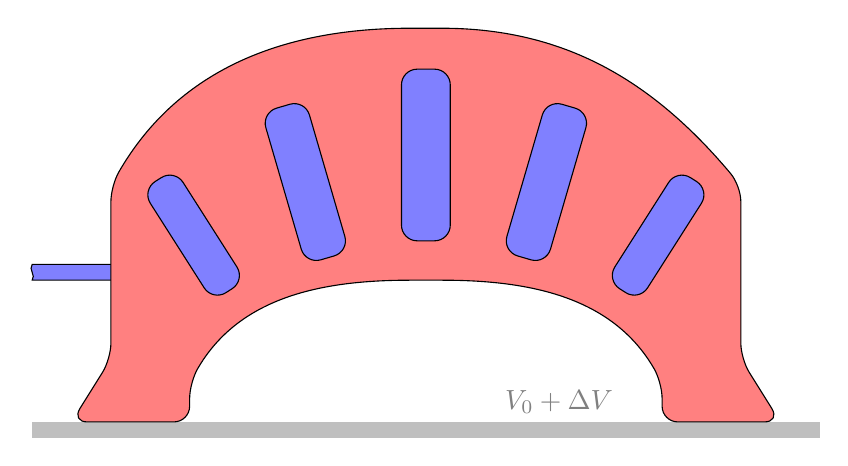
\begin{tikzpicture}[
	scale=1,
	rubber/.style={draw, fill=red!50, rounded corners=2mm},
	air/.style={draw, fill=blue!50, rounded corners=2mm},
	substrate/.style={fill=gray!50},
	inlet/.style={draw, fill=blue!50},
	notes/.style={draw, thin, gray}
]

%% Frame

%\foreach \x in {-5,-4, ...,5}{
%	\draw[help lines] (\x,-5)node[below]{\x} -- (\x,5);
%}
%\foreach \y in {-5,-4, ...,5}{
%	\draw[help lines] (-5,\y)node[left]{\y} -- (5,\y);
%}


%% Substrate
\path[substrate] (-5,0)rectangle++(10,-.2);


%% Air Inlet
\path[inlet] (-4,2)--++(-1,0)to[out=-130, in=50]++(0,-.2)--++(1,0);


%% Rubber
\path[rubber] (-4, .8)--(-4.5, 0)--(-3,0)--(-3, .5)coordinate(LI)
to[out=60, in=180] (0,1.8) to[out=0, in=120]
(3,.5)coordinate(RI)--(3,0)--(4.5, 0)--(4,.8)--(4,3)coordinate(RO) 
to[out=130, in=0](0,5)to[out=180, in=60](-4,3)--cycle
;



%% Air Channels
\def\h{1.3}
\def\b{.4}
\def\hO{1.2}
\foreach \x in {-2.5, -1.25, 0, 1.25, 2.5}{
	\pgfmathsetmacro{\x}{\x}
	\pgfmathsetmacro{\dy}{1.3 - (sqrt((\x)^2)/3)}
	\ifnum 0 = \x 
		\def\dy{1.1} 
	\fi
	\pgfmathsetmacro{\alp}{-1*(\x)*13}
	\path (\x,\hO+\dy)++(\alp+180:\b*.5+\dy*.1)coordinate(X); % node[below]{\dy};
	\path[air] (X)--++(\alp+90:\h+\dy*.8)--++(\alp:\b+\dy*.2)--++(\alp-90:\h+\dy*.8)--cycle;
}


%% Notes
\path[notes] (2.5,.25)node[left]{$V_0 + \Delta V$};



\end{tikzpicture}
\end{document}